\documentclass[10pt]{beamer}
\usepackage{amsmath}
\usepackage{amssymb}
\usepackage{geometry}
\usepackage{graphicx}
\usepackage{url}
\usepackage{bm}

\makeatletter
\let \@sverbatim \@verbatim
\def \@verbatim {\@sverbatim \verbatimplus}
{\catcode`'=13 \gdef \verbatimplus{\catcode`'=13 \chardef '=13 }} 
\makeatother

\begin{document}

%------------------------------------------
\begin{frame}
\large
Lecture 3\\
Inference for Simple Linear Regression (part 2):\\ 
Prediction Intervals\\
STAT 632, Spring 2020
\end{frame}

%------------------------------------------
\begin{frame}
Given a new value for the explanatory variable $x^*$, the prediction for the response is 
$$\hat{y}^* = \hat{\beta}_0 + \hat{\beta}_1 x^* $$\\
\vspace{10pt}

We are also interested in quantifying the uncertainty in this prediction.  That is, we are interested in constructing a prediction interval.
\end{frame}

%------------------------------------------
\begin{frame}[fragile]{Example}
\begin{itemize}
\item The R data set \texttt{trees} contains measurements of the diameter (girth), height, and volume of timber in 31 felled black cherry trees.\\
\vspace{5pt}
\item \textbf{Question}: Can the diameter of a cherry tree be used to predict its volume?  If so, what is the uncertainty associated with that prediction?
\end{itemize}

\small
\begin{verbatim}
> head(trees)
  Girth Height Volume
1   8.3     70   10.3
2   8.6     65   10.3
3   8.8     63   10.2
4  10.5     72   16.4
5  10.7     81   18.8
6  10.8     83   19.7
> dim(trees)
[1] 31  3
\end{verbatim}

\end{frame}

%------------------------------------------
\begin{frame}[fragile]
Based on the regression summary below, the equation of the least squares line is\\
$$\hat{y} = -36.9435 + 5.0659x$$

\small
\begin{verbatim}
> lm1 <- lm(Volume ~ Girth, data=trees)
> summary(lm1)

Coefficients:
            Estimate Std. Error t value Pr(>|t|)    
(Intercept) -36.9435     3.3651  -10.98 7.62e-12 ***
Girth         5.0659     0.2474   20.48  < 2e-16 ***
---
Signif. codes:  0 ‘***’ 0.001 ‘**’ 0.01 ‘*’ 0.05 ‘.’ 0.1 ‘ ’ 1

Residual standard error: 4.252 on 29 degrees of freedom
Multiple R-squared:  0.9353,	Adjusted R-squared:  0.9331 
F-statistic: 419.4 on 1 and 29 DF,  p-value: < 2.2e-16
\end{verbatim}
\end{frame}

%------------------------------------------
\begin{frame}
Given a new diameter measurement, $x^*=17$ inches, the prediction for timber volume is\\ 
$$\hat{y}^* = -36.9435 + 5.0659(17) = 49.18 \text{ ft$^3$}$$
\begin{figure}
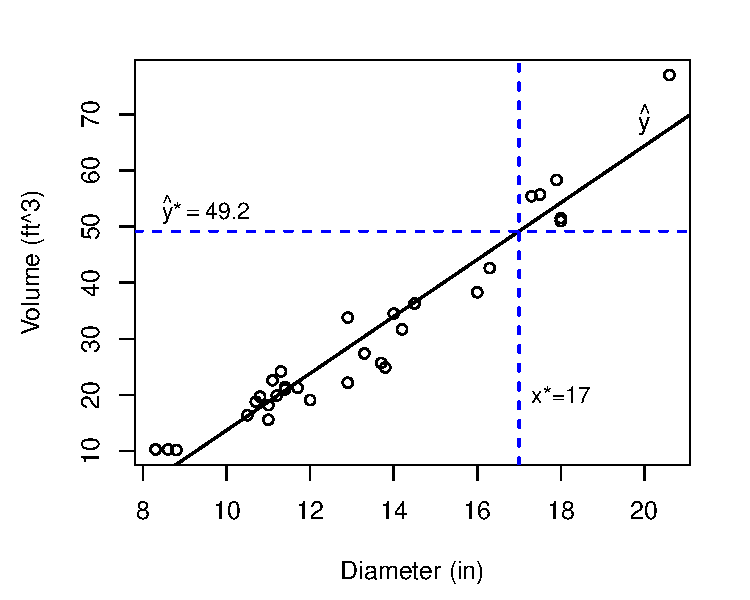
\includegraphics[scale=0.6]{figure/scatter1.pdf}
\end{figure}
\end{frame}

% \begin{frame}
% Illustration of 95\% prediction interval for the volume of a cherry tree with a measured diameter $x^* = 17$ in.
% \begin{figure}
% 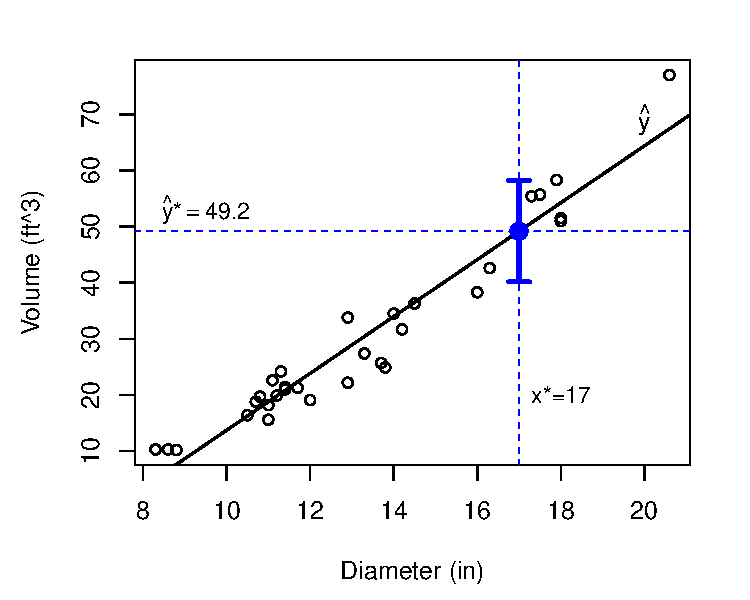
\includegraphics[scale=0.65]{figure/scatter2.pdf}
% \end{figure}
% \end{frame}

% \begin{frame}
% Illustration of 95\% prediction interval band.
% \begin{figure}
% 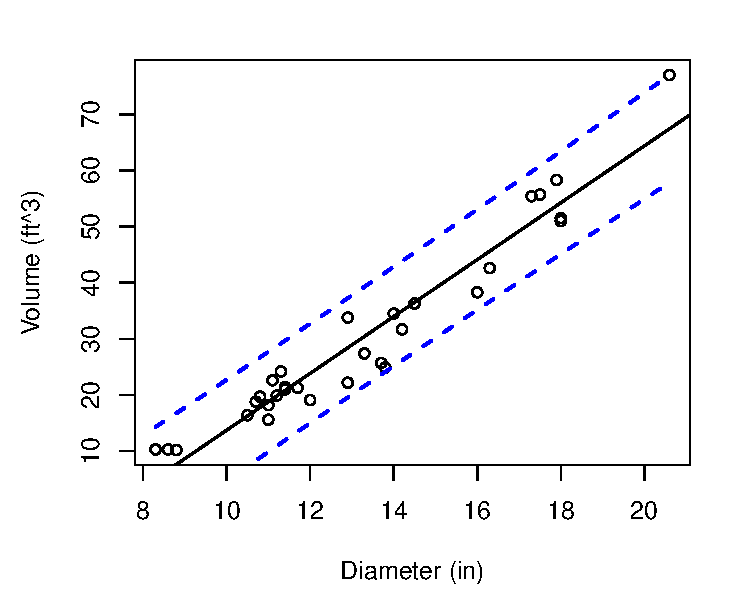
\includegraphics[scale=0.65]{figure/scatter3.pdf}
% \end{figure}
% \end{frame}

%------------------------------------------
\begin{frame}
When quantifying uncertainty, we need to distinguish between predicting the mean response and a new, actual value of the response.
\begin{itemize}
\item The mean response:
$$E(Y| X=x^*) = E(\beta_0 + \beta_1 x^* + e) = \beta_0 + \beta_1 x^*$$
For example, this represents the average volume for cherry trees that have an $x^*=17$ inch diameter.  Note that the mean response is fixed (non-random) since $\beta_0$ and $\beta_1$ are population parameters.
\vspace{10pt}
\item A new, actual value of the response:
$$Y^* = \beta_0 + \beta_1 x^* + e \text{, where } e \sim N(0,\sigma^2)$$ 
For example, this represents the volume for a single cherry tree that has an  $x^*=17$ inch diameter.  Note that $Y^*$ is defined here as a random variable.
\end{itemize}
\end{frame}

% \begin{frame}{Notation}
% \begin{itemize}
% \item $X$ and $Y$ are random variables.
% \item $x$ and $y$ refer to specific values.
% \item $x_i$ and $y_i$ refer to specific values from a collection of $i=1, \cdots, n$ observations.
% \item $\hat{y}^* = \hat{\beta}_0 + \hat{\beta}_1 x^*$ is the prediction of the response at a new, specific value of the explanatory variable $x^*$.
% \item $Y^* = \beta_0 + \beta_1 x^* + e$ is a random variable representing the response variable for given $x^*$.
% \end{itemize}
% \end{frame}

%------------------------------------------
\begin{frame}{Confidence interval for the mean response}
When constructing a confidence interval for the mean response there is only one source of variability: the estimation of the population parameters ($\beta_0$ and $\beta_1$).
\begin{align*}
Var(\hat{y}^*) = Var(\hat{\beta}_0 + \hat{\beta}_1 x^*)
&= \sigma^2 \left[ \frac{1}{n} + \frac{(x^* - \bar{x})^2}{\text{SXX}} \right],
\end{align*}
where SXX $= \sum_{i=1}^n (x_i - \bar{x})^2$.
\end{frame}
% write formula for mean response on board

%------------------------------------------
\begin{frame}{Confidence interval for the mean response}
A 1-$\alpha$ confidence interval for the mean response:
$$\hat{y}^* \pm t_{\alpha/2; n-2} \hat{\sigma} \sqrt{\frac{1}{n} + \frac{(x^* - \bar{x})^2}{ \text{SXX}}},$$
where $\hat{y}^* = \hat{\beta}_0 + \hat{\beta}_1 x^*$, and $\hat{\sigma}$ is the residual standard error.\\
\vspace{15pt}

The interpretation is ``We are 95\% confident that the mean response is between ..."
\end{frame}

%------------------------------------------
\begin{frame}[fragile]{Example - R Computation}
Use R to calculate a 95\% confidence interval for the mean volume of cherry trees that have diameter $x^* = 17$ inches.

\begin{verbatim}
> new_x <- data.frame(Girth = 17)
> predict(lm1, newdata = new_x, interval="confidence")
      fit      lwr      upr
1 49.1761 46.71799 51.63421
\end{verbatim}

The interpretation is that the predicted mean volume, for cherry trees that have a 17 inch diameter, is 49.18 cubic feet.  Additionally, we are 95\% confident that the population mean volume, for cherry trees that have a 17 inch diameter, is between 46.72 and 51.63 cubic feet.    
\end{frame}

%------------------------------------------
\begin{frame}{Example - Illustration}
A 95\% confidence interval for mean volume of cherry trees that have a 17 inch diameter. 
\begin{figure}
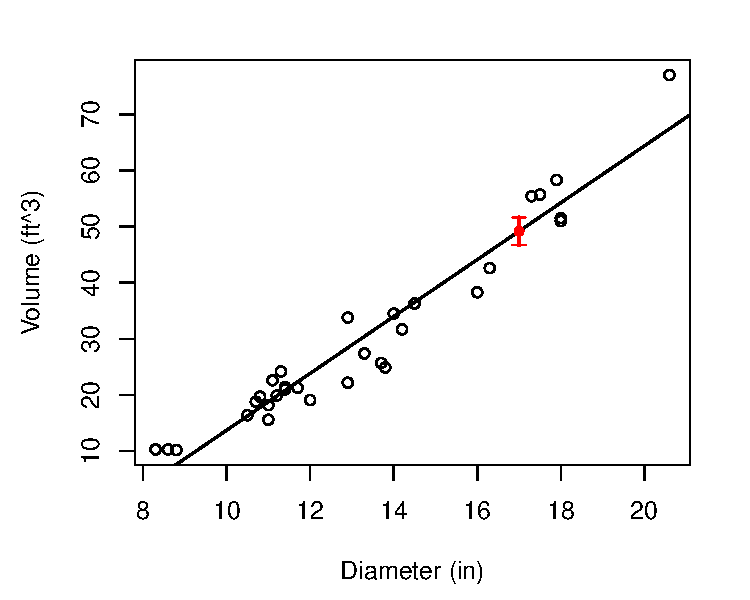
\includegraphics[scale=0.65]{figure/scatter4.pdf}
\end{figure}
\end{frame}

%------------------------------------------
\begin{frame}{Example - Illustration}
A 95\% confidence band (or envelope) for mean timber volume.  We can also think of this as a confidence band for the population regression line.
\begin{figure}
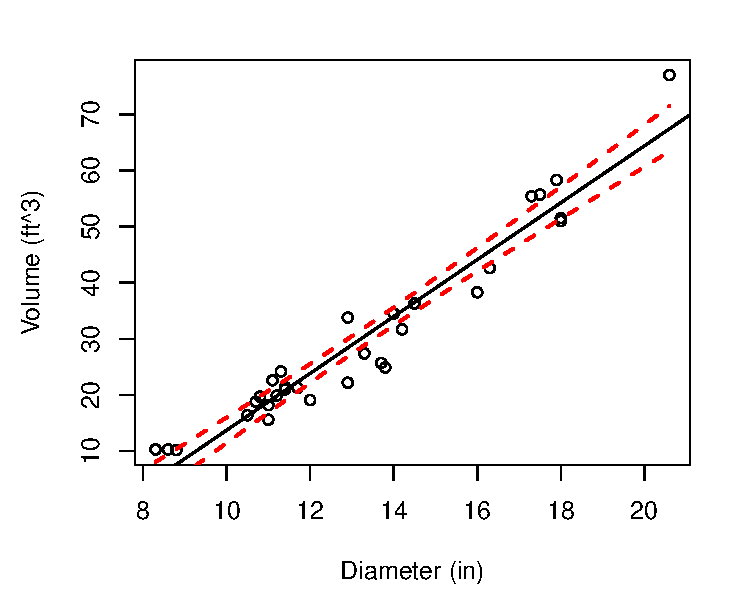
\includegraphics[scale=0.65]{figure/scatter5.pdf}
\end{figure}
\end{frame}

%------------------------------------------
\begin{frame}[fragile]{Example - Illustration}
A 95\% confidence band using \texttt{ggplot2}.
\begin{verbatim}
ggplot(trees, aes(Girth, Volume)) +
  geom_point() + stat_smooth(method = "lm", se = TRUE) +
  xlab("Diameter (in)") + ylab("Volume (ft^3)")
\end{verbatim}
\begin{figure}
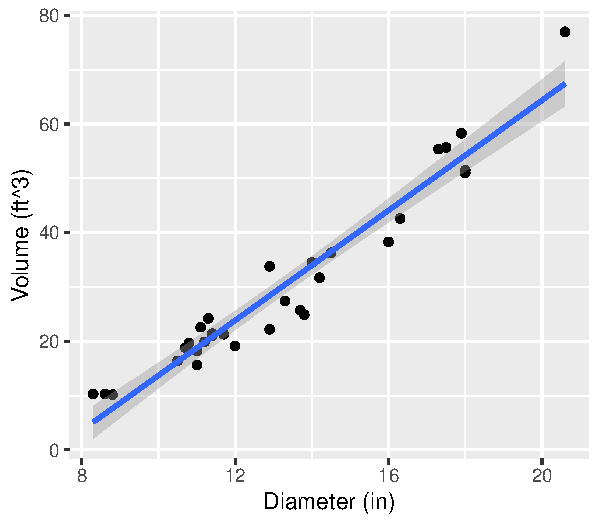
\includegraphics[scale=0.55]{figure/ggplot_ci.pdf}
\end{figure}
\end{frame}

%------------------------------------------
\begin{frame}{Prediction interval for an actual response value}
When constructing a prediction interval for a new, actual value of the response there are two sources of variability: the estimation of the population parameters ($\beta_0$ and $\beta_1$), and the random error $e$. 
\begin{align*}
Var(\hat{y}^* + e) &= Var(\hat{\beta}_0 + \hat{\beta}_1 x^*) + Var(e)\\
&= \sigma^2 \left[ 1 + \frac{1}{n} + \frac{(x^* - \bar{x})^2}{\text{SXX}} \right],
\end{align*}
where SXX $= \sum_{i=1}^n (x_i - \bar{x})^2$.\\
\end{frame}
% write formula for new, actual value of the response on board

%------------------------------------------
\begin{frame}{Prediction interval for an actual response value}
A 1-$\alpha$ prediction interval for a new, actual value of the response:
$$\hat{y}^* \pm t_{\alpha/2; n-2} \hat{\sigma} \sqrt{1 + \frac{1}{n} + \frac{(x^* - \bar{x})^2}{\text{SXX}}},$$
where $\hat{y}^* = \hat{\beta}_0 + \hat{\beta}_1 x^*$, and $\hat{\sigma}$ is the residual standard error.\\
\vspace{15pt}

The interpretation is ``A 95\% prediction interval for the response is ..."
\end{frame}

%------------------------------------------
\begin{frame}[fragile]{Example - R Computation}
Use R to construct a 95\% prediction interval for the volume of a single cherry tree that has diameter $x^* = 17$ inches.

\begin{verbatim}
> new_x <- data.frame(Girth = 17)
> predict(lm1, newdata = new_x, interval="prediction")
      fit      lwr      upr
1 49.1761 40.13908 58.21312
\end{verbatim}

The interpretation is that the predicted volume, for a cherry tree that has a 17 inch diameter, is 49.18 cubic feet.  Additionally, the 95\% prediction interval is between 40.14 and 58.21.  This means that the actual volume of a cherry tree, with a 17 inch diameter, is likely to be between 40.14 and 58.21 cubic feet.    
\end{frame}

\begin{frame}{Example - Illustration}
95\% prediction interval for the volume of a cherry tree with diameter $x^*=17$ in.
\begin{figure}
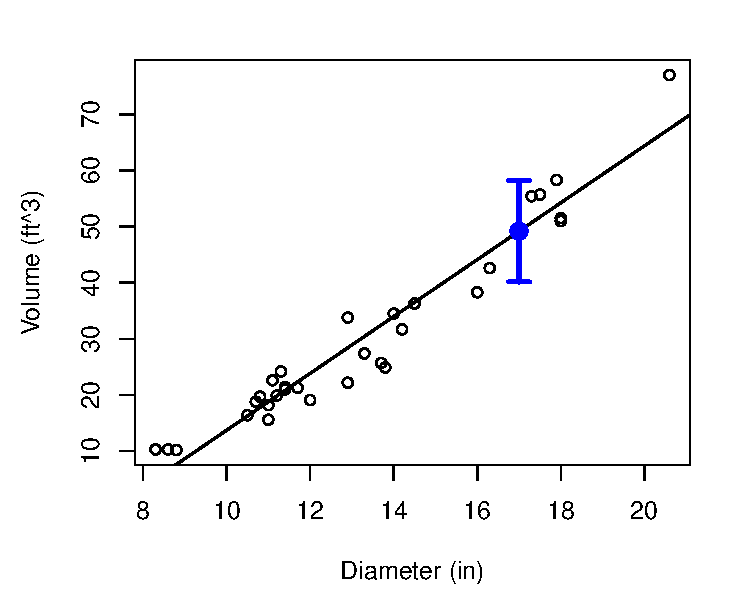
\includegraphics[scale=0.65]{figure/scatter6}
\end{figure}
\end{frame}

\begin{frame}{Example - Illustration}
95\% prediction interval band.
\begin{figure}
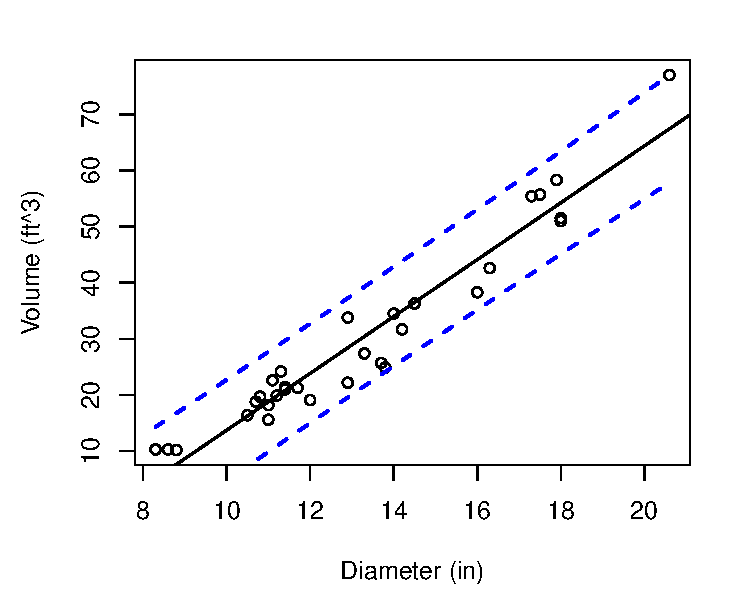
\includegraphics[scale=0.65]{figure/scatter3}
\end{figure}
\end{frame}

\begin{frame}[fragile]
Here is the R code for the previous figure:
\small
\begin{verbatim}
> lm1 <- lm(Volume ~ Girth, data=trees)
> plot(Volume ~ Girth, xlab='Diameter (in)', 
       ylab = 'Volume (ft^3)', data=trees, cex=0.9)
> abline(lm1, lwd=1.5)
> min_x <- min(trees$Girth)
> max_x <- max(trees$Girth)
> grd_x <- seq(min_x, max_x, by=0.1)
> new_x <- data.frame(Girth = grd_x)
> PI <- predict(lm1, newdata = new_x, interval="prediction")
> PI <- as.data.frame(PI)
> lines(grd_x, PI$lwr, lty=2, lwd=2, col="blue")
> lines(grd_x, PI$upr, lty=2, lwd=2, col="blue")
\end{verbatim}
\end{frame}

\begin{frame}[fragile]
We can also change the confidence level.  Note that 95\% is the default.\\
\vspace{10pt}

\begin{verbatim}
> new_x <- data.frame(Girth = 17)
> predict(lm1, newdata = new_x, 
    interval="prediction", level=0.99)
      fit      lwr      upr
1 49.1761 36.99677 61.35543
\end{verbatim}

\end{frame}

\begin{frame}[fragile]{Comparing PIs and CIs}
\begin{verbatim}
> new_x <- data.frame(Girth = 17)
> predict(lm1, newdata = new_x, interval="confidence")
      fit      lwr      upr
1 49.1761 46.71799 51.63421
> predict(lm1, newdata = new_x, interval="prediction")
      fit      lwr      upr
1 49.1761 40.13908 58.21312
\end{verbatim}

\begin{itemize}
\item The point predictions for the mean response and an actual value of the response are the same ($\hat{y}^* = 49.176$ when $x^*=17$).
\item The prediction interval for the actual response is substantially wider than the confidence interval for the mean response.
\end{itemize}
\end{frame}

\begin{frame}{Comparing PIs and CIs}
The 95\% prediction interval band is wider than the confidence interval band.
\begin{figure}
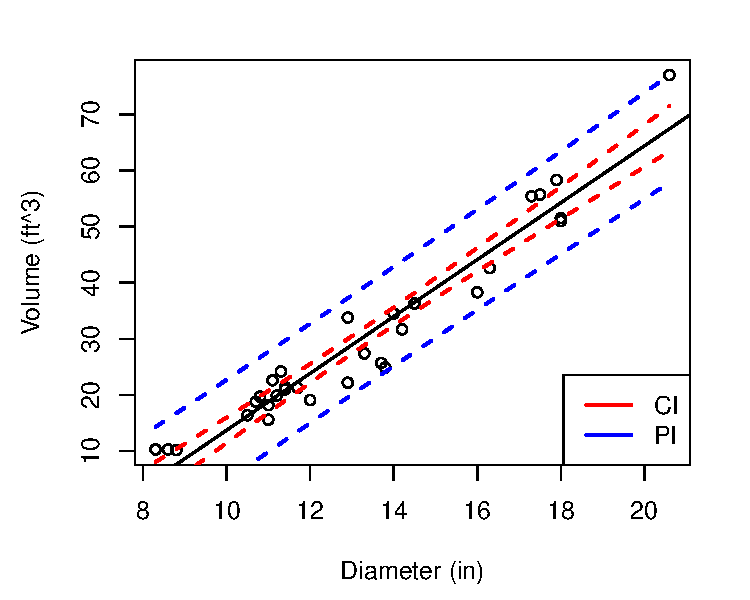
\includegraphics[scale=0.65]{figure/scatter7.pdf}
\end{figure}
\end{frame}
%split into 2 slides

\begin{frame}{Diagnostics?}
When making inferences we should also check that the conditions for SLR are satisfied (linearity, constant variance, independence, normality).  One useful diagnostic is a plot of the residuals versus the fitted values.
\begin{figure}
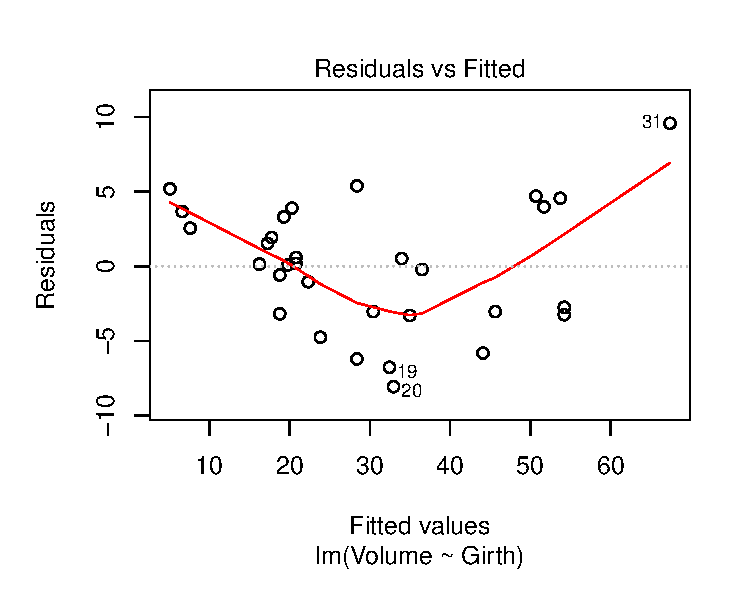
\includegraphics[scale=0.45]{figure/resid.pdf}
\end{figure}
There is obvious curvature in the residuals.  Transformations or incorporating quadratic effects might improve the model (topics for future lectures). 
\end{frame}

\begin{frame}{Summary}
\begin{itemize}
\item In addition to using SLR to make a prediction for the response variable, we can also construct a prediction interval that quantifies the uncertainty in that prediction.\\
\vspace{10pt}
\item It is important to distinguish between a confidence interval for the mean response and a prediction interval for the actual response.\\
\vspace{10pt}
\item Prediction intervals are more useful and common in practice. 
\end{itemize}
\end{frame}
%PIs are generally more useful the CI
%HW/Exams assignments will focus more PIs


\end{document}